\documentclass[a4paper]{article}

\usepackage{geometry}
\usepackage{natbib}
\bibpunct[:]{(}{)}{,}{a}{}{;}

%--------------------
%\usepackage{gb4e}
%\noautomath

\usepackage{amsmath}
\usepackage{amsfonts}
\usepackage{amsthm}
\usepackage{amssymb}
\usepackage{mathrsfs}
\usepackage{nicefrac}
%\usepackage{stmaryrd}
%\usepackage{multicol}
\usepackage{graphicx}
\usepackage{color}
\usepackage{booktabs}

\usepackage{caption}
\usepackage{subcaption}

%\newcommand{\mvalueof}[1]{\llbracket#1\rrbracket}
\newcommand{\citeposs}[2][]{\citeauthor{#2}'s (\citeyear[#1]{#2})}
\newcommand{\tuple}[1]{\ensuremath{\left\langle #1 \right\rangle}} 

\newcommand{\hl}[1]{\textcolor[rgb]{.8,.33,.0}{#1}}% prints in orange
%\newcommand{\argmax}[1]{\underset{#1}{\operatorname{arg}\,\operatorname{max}}\;}
%\newcommand{\argmin}[1]{\underset{#1}{\operatorname{arg}\,\operatorname{min}}\;}
%\newcommand{\sbna}{\exists\lnot\forall}

\definecolor{Red}{RGB}{178,34,34}
\newcommand{\mf}[1]{\textcolor{Red}{[MF: #1]}} 
\newcommand{\tb}[1]{\textcolor[rgb]{.8,.33,.0}{[TB: #1]}}% prints in orange

\usepackage{blkarray}
\usepackage{xspace}

%%% MF's commands
\newcommand{\set}[1]{\left\{#1\right\}}
\newcommand{\card}[1]{\left \lvert \, #1 \, \right\rvert}
\newcommand{\abs}[1]{\lvert #1 \rvert}
\newcommand{\States}{\ensuremath{S}\xspace}		% Set of States
\newcommand{\state}{\ensuremath{s}\xspace}		% single states
\newcommand{\mystate}[1]{\ensuremath{\state_{\text{#1}}}\xspace} %meaningful states
\newcommand{\Messgs}{\ensuremath{M}\xspace}		% Set of Messages
\newcommand{\messg}{\ensuremath{m}\xspace}		% single messages
\newcommand{\mymessg}[1]{\ensuremath{\messg_{\text{#1}}}\xspace} %meaningful messages
\newcommand{\ssome}{\mystate{\ensuremath{\exists\neg\forall}}}
\newcommand{\sall}{\mystate{\ensuremath{\forall}}}
\newcommand{\snone}{\mystate{\ensuremath{\emptyset}}}
\newcommand{\msome}{\mymessg{some}}
\newcommand{\mall}{\mymessg{all}}
\newcommand{\mnone}{\mymessg{none}}
\newcommand{\asome}{\myact{\ensuremath{\exists\neg\forall}}}
\newcommand{\aall}{\myact{\ensuremath{\forall}}}
\definecolor{mygray}{cmyk}{0.35,0.35,0.35,0.35}
\newcommand{\mygray}[1]{{\textcolor{mygray}{#1}}}
%%% 


%--------------------
%
%\usepackage{setspace}
%\onehalfspacing
%
%-------------------


\title{Tracing the cultural evolution of meaning at the semantics-pragmatics interface}

\author{%\bf NAME1 and NAME2\\
    ( -- draft \today --- )
}


\date{}

\begin{document}

We consider three states $\States = \set{\snone, \ssome, \sall}$. This state space can be
thought of as a partition of possible worlds into cells where none, some or all of the $A$s are
$B$s, for some arbitrary fixed predicates $A$ and $B$. Eight concepts can be distinguished
based on their truth or falsity in three world states, six of which are not contradictory
(always false) or tautologous (always true). These are listed with mnemonic names in
Table~\ref{tab:concepts}. 

\begin{table}
  \centering
\begin{center}
  \begin{tabular}{lccclc}
    \toprule
    intuitive name
    & \snone
    & \ssome
    & \sall
    & least complex formula
    & complexity
    \\ \midrule
    ``all''
    & 0
    & 0
    & 1
    & $A \subseteq B$
    & $3$
    \\
    ``some but not all''
    & 0
    & 1
    & 0
    & $A \cap B \neq \emptyset \wedge A \neq \emptyset$
    & $8$
    \\    
    ``some''
    & 0
    & 1
    & 1
    & $A \cap B \neq \emptyset$
    & $4$
    \\
    ``none''
    & 1
    & 0
    & 0
    & $A \cap B = \emptyset$
    & $4$
    \\
    ``none or all''
    & 1
    & 0
    & 1
    & $\neg(A \cap B \neq \emptyset \wedge A \neq \emptyset)$
    & \tb{$10$}
    \\
    ``not all''
    & 1
    & 1
    & 0
    & $\neg (A \subseteq B)$
    & $5$
    \\
    \bottomrule
  \end{tabular}
\end{center}
\caption{Available concepts and their minimal derivation length}
\label{tab:concepts}
\end{table}

A lexicon $L$ is a mapping $\Messgs \rightarrow C$ from messages to concepts. With three
messages there are $6^3 = 216$ possible lexica, but many of these assign the same concept to
more than one message. For simplicity, we restrict attention to only those lexica which avoid
expressive redundancy. Hardcoding such an \emph{mutual exclusivity bias}
\citep[e.g.][]{Clark2009:Lexical-Meaning}, there are 20 non-redundant lexica. Functional
pressure towards efficient communication will evidently favor non-redundant lexica, so this
restriction is fairly innocuous but practical.

As before, the type of a player is a combination of a lexicon and a manner of pragmatic
language use: literal or pragmatic. With this, there are 40 types in this model.

\begin{table}
  \centering
  \begin{align*}
    C & \rightarrow_2 C \wedge C 
    & 
    X & \rightarrow_1 \set{A,B} \\
    C & \rightarrow_2 \neg C 
    & 
    X & \rightarrow_1 X \cap X \\
    C & \rightarrow_1 X \subseteq X
    & 
    X & \rightarrow_1 X \cup X \\
    C & \rightarrow_1 X \neq \emptyset \\
    C & \rightarrow_1 X = \emptyset     
  \end{align*}
  \caption{Toy grammar in a set-theoretic "language of thought"}
  \label{tab:grammar}
\end{table}


The prior probability of a type is just the prior probability of its lexicon. The prior of a
lexicon is a function of the complexity of the concepts in its image set. Lexica that use
simpler concepts are \emph{a priori} more likely. This can be motivated by assuming that
learners beam search for suitable concepts to map onto overt signals by (probabilistically)
considering simpler concepts first. Many ways for defining complexity of a concept are
conceivable. If strong empirical claims were at stake here, empirically motivated measures of
complexity should be used. For the sake of a non-trivial example, we follow
\citet{piantadosi+etal:underreview} and related work to define complexity of a concept as a
function of its derivation cost in a (weighed or probabilistic) generative ``language of
thought''. For concreteness of example, consider the toy grammar of concepts in
Table~\ref{tab:grammar}. This grammar uses basic set-theoretic operations to form expressions
which can be evaluated as true or false in our three world states. Applications of generative
rules have a cost attached to them. (Alternatively, a probability.) Here we simply assume that
Boolean combinations of concepts are more complex than ``atomic'' concepts and that otherwise
each rule application adds the same cost unit. Table~\ref{tab:concepts} lists, for each
concept, the least complex formula derivable in this grammar that has the appropriate truth
conditions. A simple way of defining priors over a lexicon is:
\begin{align*}
  P(L)  & = \prod_{c \in Im(L)} P(c)  \ \ \ \text{, with} & 
  P(c) & \propto \max_{c'}Compl(c') - Compl(c') + 1\,,
\end{align*}
where $Compl(c)$ is the complexity of each concepts. \tb{I changed `$P(L) = $' to `$P(L) \propto$', as well as   `$P(c) \propto \max_{c'}Compl(c') - Compl(c) + 1$'. I hope both were intended like this}.

\section*{Some results} To get an idea of how this changes our previous results, I inspected some of the new setup's properties. Overall, the results are quite similar. A couple remarks: 
\begin{enumerate}
\item So far there is no parameter to regulate the strength of the inductive bias (before controlled by $c$). This means that we could get stronger/weaker results than the ones presented here
\item Our target type is $t_{24}$, made explicit below, which currently has (i) the most a priori probable lexicon (see Figure \ref{fig:priors}), but is (ii) not the most learnable (see Figure \ref{fig:q-matrices}), nor (iii) the fittest type (see Figure \ref{fig:u-matrix}). 
\item In terms of the dynamics, $t_{24}$ fares worse than in our target type in the previous setup under only replication, OK but far from perfectly under mutation, but fares surprisingly well under when both dynamics are involved (see Figure \ref{fig:outcomes})
\item Functional deficiency of $t_{24}$ is due to its (Gricean) receiver behavior. In principle, this would not be so if either (i) receivers were one level higher in the reasoning type hierarchy or (ii) receivers soft-maximized.
\item As noted earlier by Michael, having our target be the most a priori probable is not so nice. On the other hand, we could stress the fact that its not the most communicatively efficient nor the most learnable language (when learning from a parent of the same type). 
\item Overall, this seems to work. We have a lot more types and more complex lexica but the results are roughly the same even without involving parameter $c$. The most important issue is to settle on a good way to transform a LOT-like representation into a prior over lexica. Personally, I'm torn between a probabilistic conception (skipping complexity and considering the probability of each rule application directly) and something akin to what Michael proposed here. I'll read up more on how other people have done it in the past in the meantime. Let me know if you have suggestions about this. Afterwards, I can run a more proper analysis.
\end{enumerate}

\section*{Details for mutual exclusivity type space}

Our target, Gricean $t_{24}$ lexicalizes messages corresponding to the \sall, \snone and \{\sall,\ssome\} (cf. Table \ref{tab:concepts}). Its lexicon is accordingly (same as literal player $t_4$):

\begin{centering}
\bordermatrix{~ &	  \mall & \msome & \mnone \cr 
                  \snone &  0 & 0 & 1 \cr
                  \ssome & 0 & 1 & 0 \cr
		  \sall & 1 & 1 & 0 \cr}
\end{centering}

Following the setup above and the complexity values in Table \ref{tab:concepts}, the priors of our $40$ types are shown here:

\begin{figure}[h!]
  \centering
  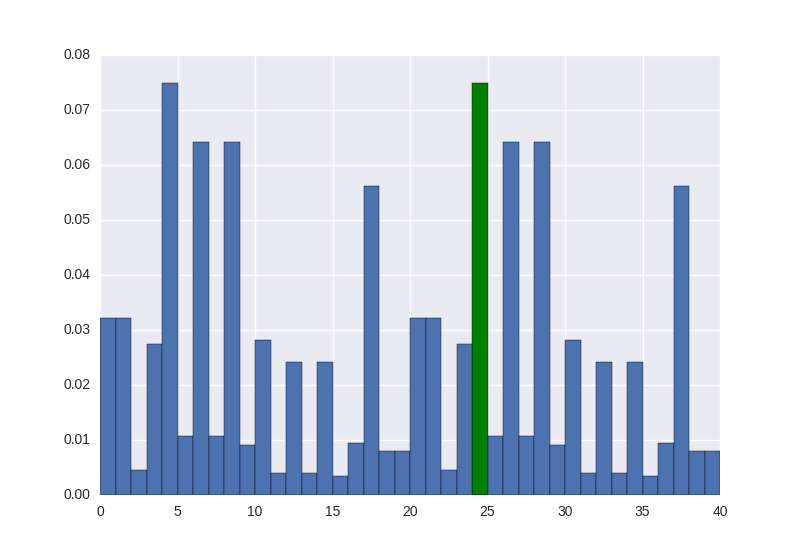
\includegraphics[scale=.35]{../code-LOT-extension/plots/priors-meTrue.png} %width = 0.75\linewidth
  \caption{Prior over types (lexica). The green prior corresponds to $t_{24}$.}
  \label{fig:priors}
\end{figure}

I thought it would be instructive to inspect different fitness and Q-matrices. As before, the matrix for expected utility only depends on parameters $\alpha$ and $\lambda$. There do not seem to be any particular surprises; $t_{24}$ is not the best but also far from the worse (see remark 4 above). With $\alpha = 1$ and $\lambda = 30$ we get $\text{EU}(t_{24},t_{24}) \approx .88$. Here's a visualization of the entire u-matrix:

\begin{figure}[h!]
  \centering
  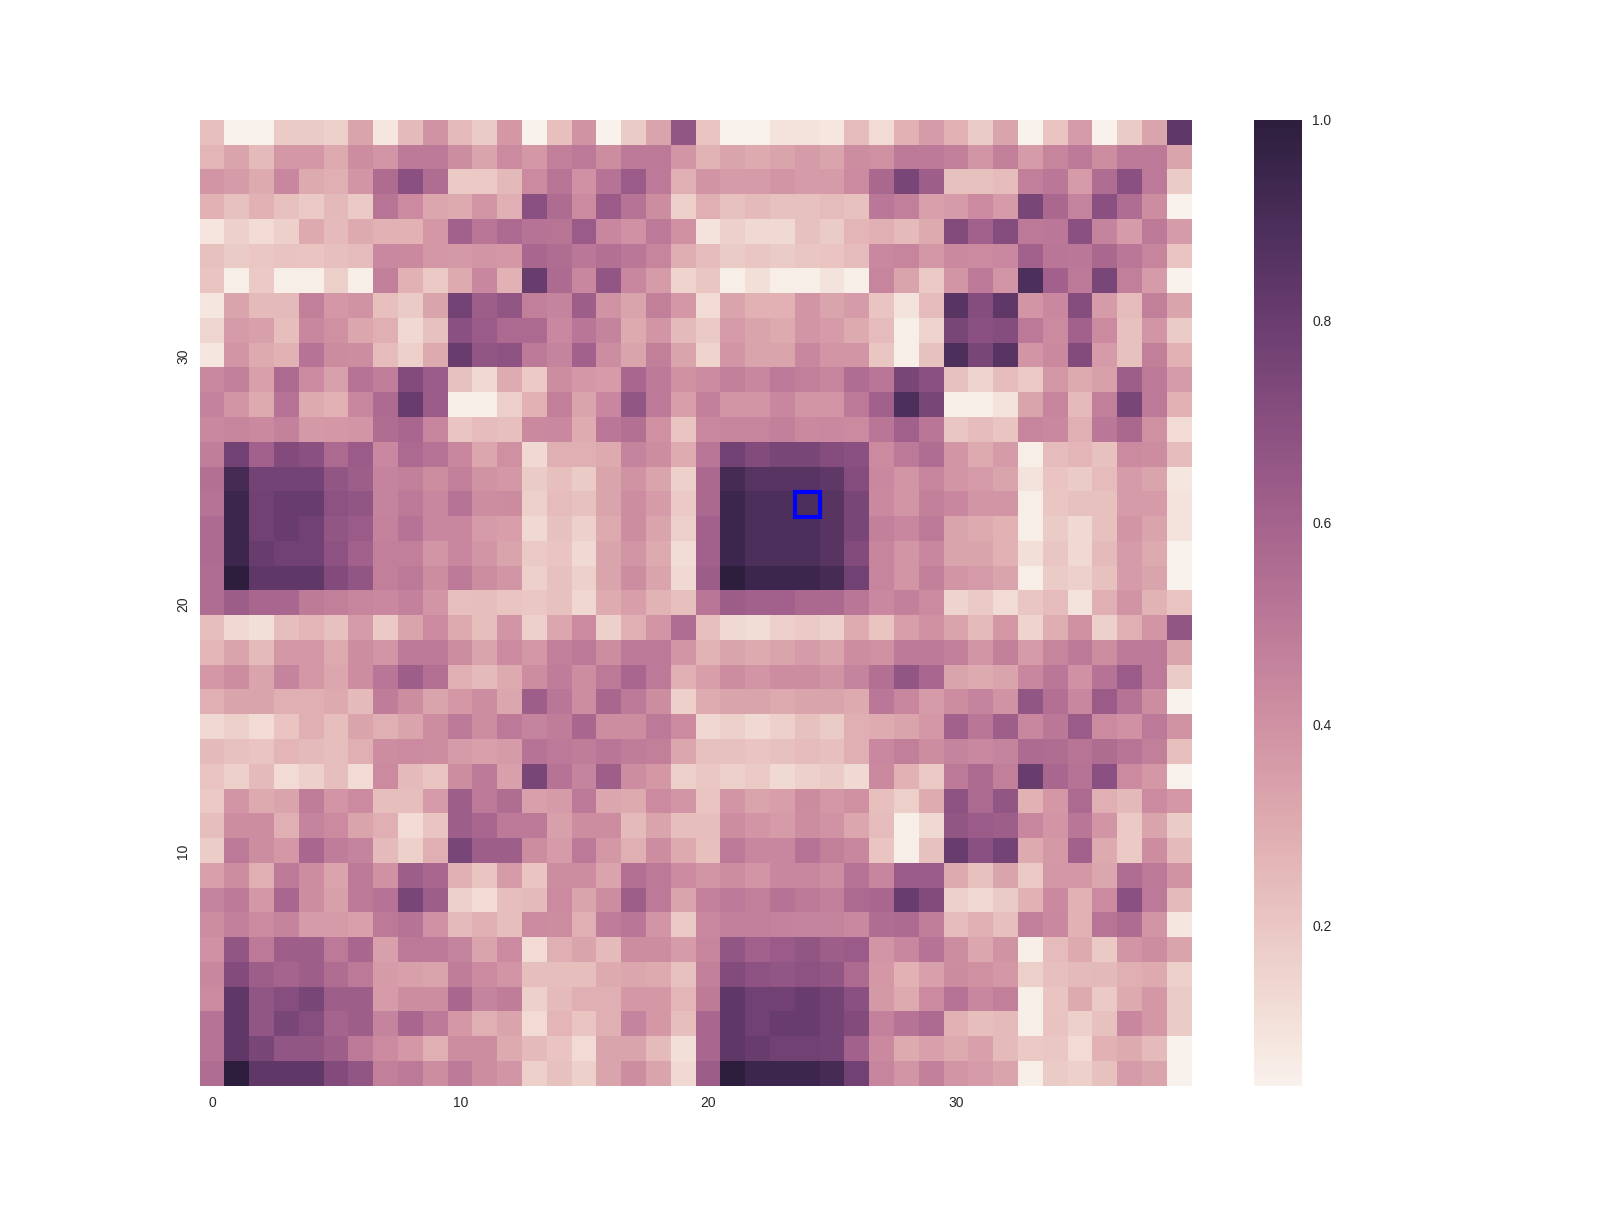
\includegraphics[scale=.25]{../code-LOT-extension/plots/u-l30-a1-meTrue.png} %width = 0.75\linewidth
  \caption{Utility-Matrix for $\alpha = 1$ and $\lambda = 30$. The boxed value corresponds to $\text{EU}(t_{24},t_{24})$.}
  \label{fig:u-matrix}
\end{figure}

For $Q$ there are more values to test. For sequence length $k$ there's not that much change as long as it is not too small and possible noise due to the sampling of learning data is accounted for (it's still important, but I'll background this for now). As before, the posterior parameter $l$ is very important. If $l \geq 10$ we get very faithful transmission of our target type. Lower values lead to more mutation. Here's a visual impression of two $Q$ matrices for different $l$ values:
\begin{figure}[h!]
  \centering
  \begin{subfigure}[b]{0.45\textwidth}
    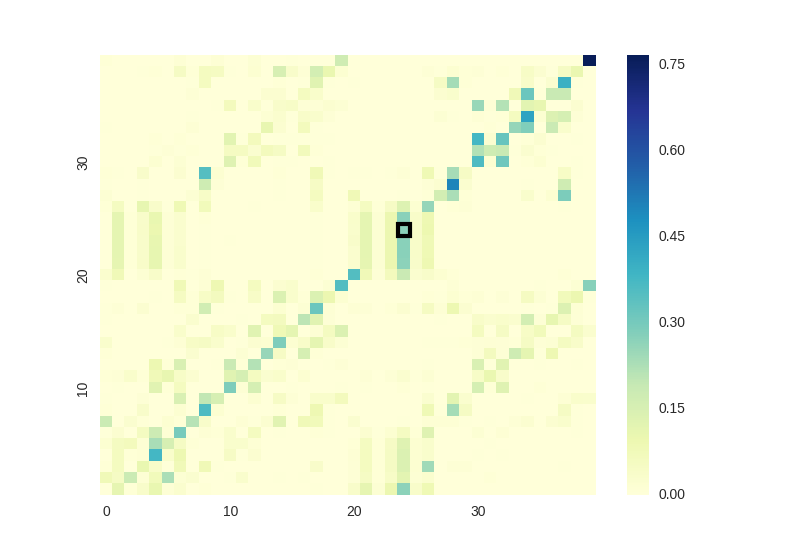
\includegraphics[scale=0.4]{../code-LOT-extension/plots/q-l30-a1-k5-l1-meTrue.png}
  \end{subfigure}
  ~
   \begin{subfigure}[b]{0.45\textwidth}
    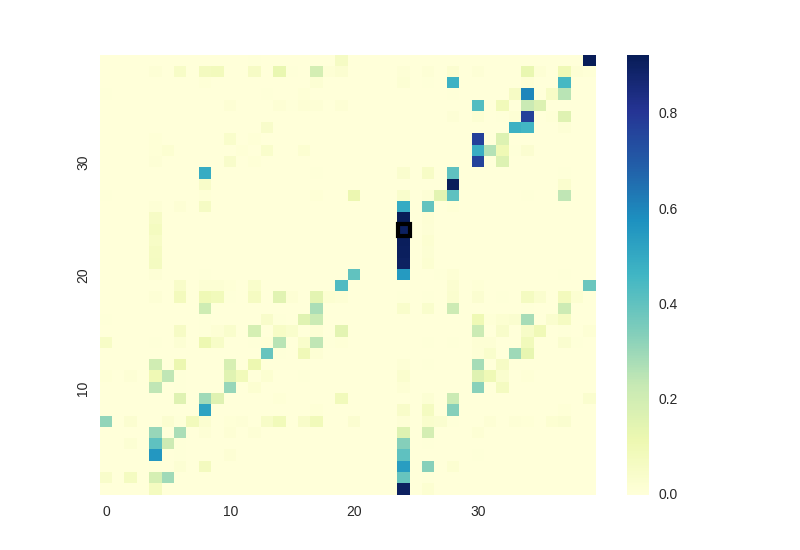
\includegraphics[scale=0.4]{../code-LOT-extension/plots/q-l30-a1-k5-l10-meTrue.png}
  \end{subfigure}
  \caption{$Q$-matrices for $\alpha = 1, \lambda = 30, k = 5$, $200$ samples per parent type with either $l = 1$ (left) and $l = 10$ (right). The boxed value corresponds to $P(t_{24} | t_{24})$.}
  \label{fig:q-matrices}
\end{figure}

\newpage

Finally, we can see how the above affects actual applications of only replication, only mutation, and replication \emph{and} mutation using the matrices shown above. To construct these plots I took the mean top $3$ types from $1000$ simulations using either of the three dynamics. If $t_{24}$ was not in the top $3$, I took out the third most prolific type and added $t_{24}$ instead. 

\begin{figure}[h!]
  \centering
  \begin{subfigure}[b]{0.45\textwidth}
    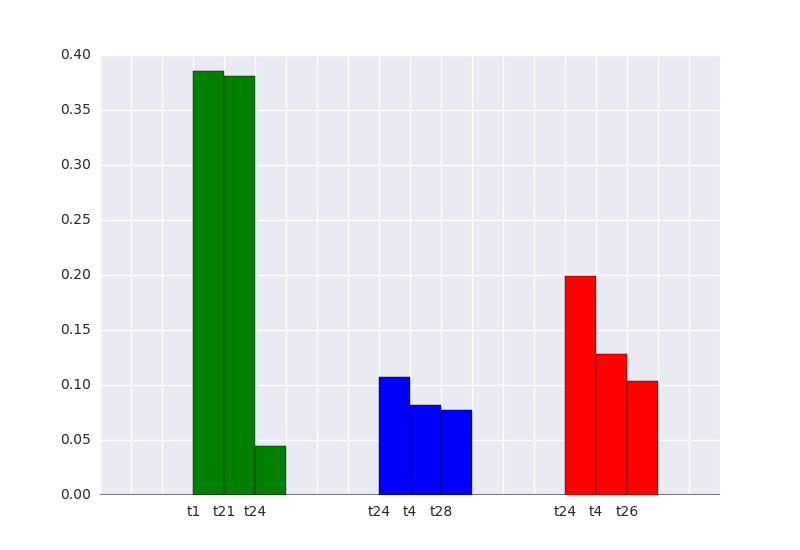
\includegraphics[scale=0.4]{../code-LOT-extension/plots/rmd-lam30-a1-k5-s200-l1-meTrue.png}
  \end{subfigure}
  ~
   \begin{subfigure}[b]{0.45\textwidth}
    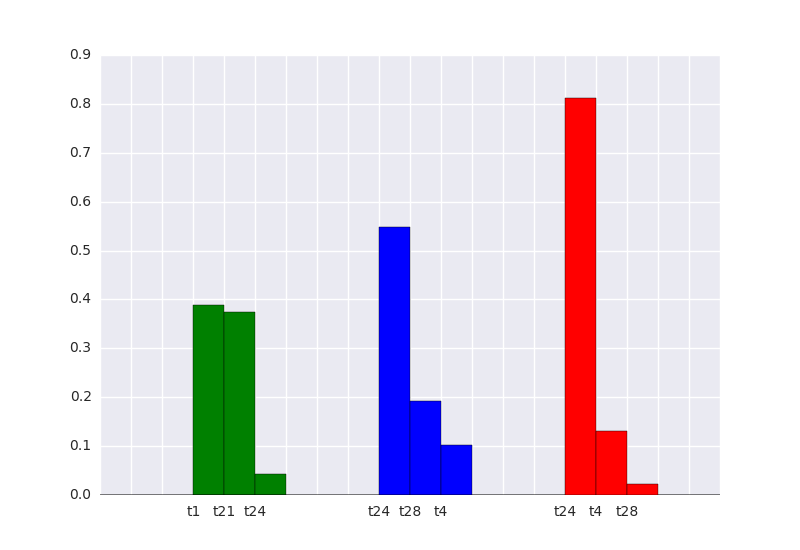
\includegraphics[scale=0.4]{../code-LOT-extension/plots/rmd-lam30-a1-k5-s200-l10-meTrue.png}
  \end{subfigure}
  \caption{Mean proportion of top $2/3$ types and target $t_{24}$ under replication only (green plot), mutation only (blue plot), and replication {\em and} mutation (red plot) after $50$ generations with $\alpha = 1, \lambda = 30, k = 5$, $200$ samples per parent type and $l = 1$ (left figure) and $l = 10$ (right figure).}
  \label{fig:outcomes}
\end{figure}

\newpage

\section*{Details for larger type space}

Our target is now Gricean $t_{68}$ with the same lexicon as $t_{24}$ in the reduced type space. Following the setup above and the complexity values in Table \ref{tab:concepts}, the priors of our now $112$ types are shown here:

\begin{figure}[h!]
  \centering
  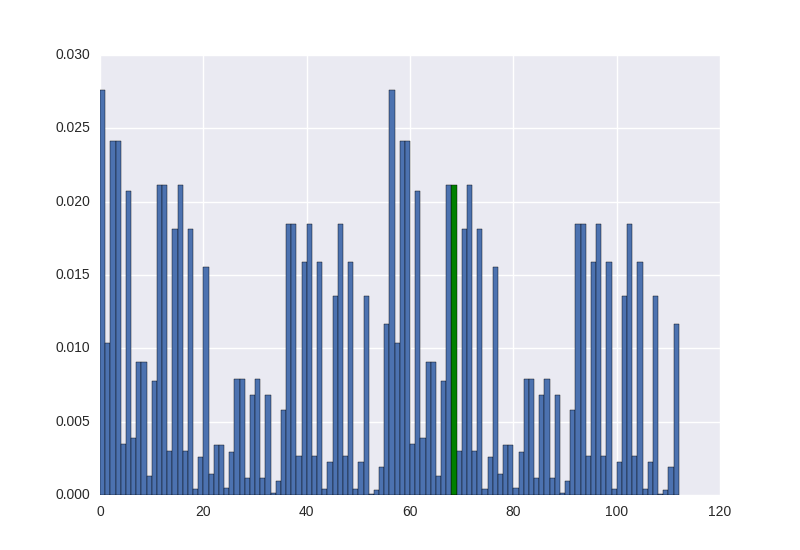
\includegraphics[scale=.35]{../code-LOT-extension/plots/priors-meFalse.png} %width = 0.75\linewidth
  \caption{Prior over types (lexica). The green prior corresponds to $t_{68}$.}
  \label{fig:priors}
\end{figure}

As before,  $t_{68}$ is not the best but also far from the worse. Here's a visualization of the entire u-matrix:

\begin{figure}[h!]
  \centering
  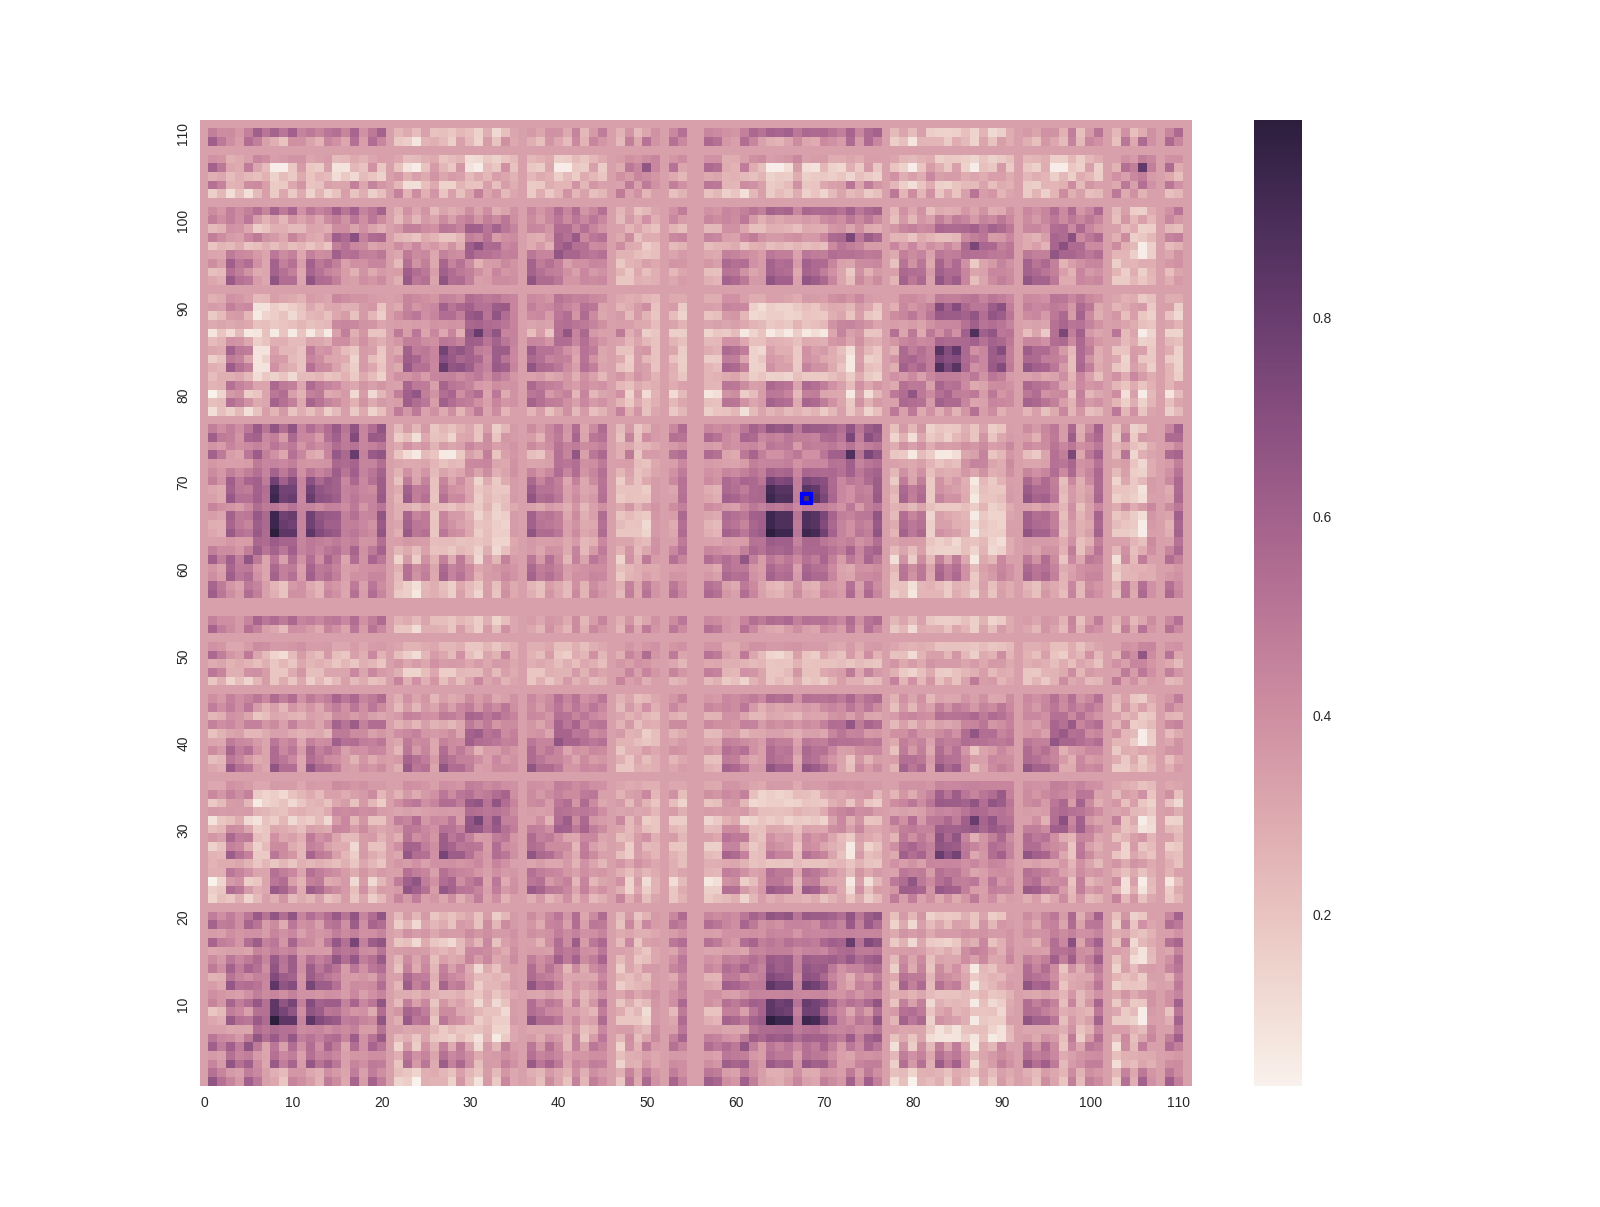
\includegraphics[scale=.25]{../code-LOT-extension/plots/u-l30-a1-meFalse.png} %width = 0.75\linewidth
  \caption{Utility-Matrix for $\alpha = 1$ and $\lambda = 30$. The boxed value corresponds to $\text{EU}(t_{68},t_{68})$.}
  \label{fig:u-matrix}
\end{figure}

Here's a visual impression of two $Q$ matrices for different $l$ values with the larger type space:

\begin{figure}[h!]
  \centering
  \begin{subfigure}[b]{0.45\textwidth}
    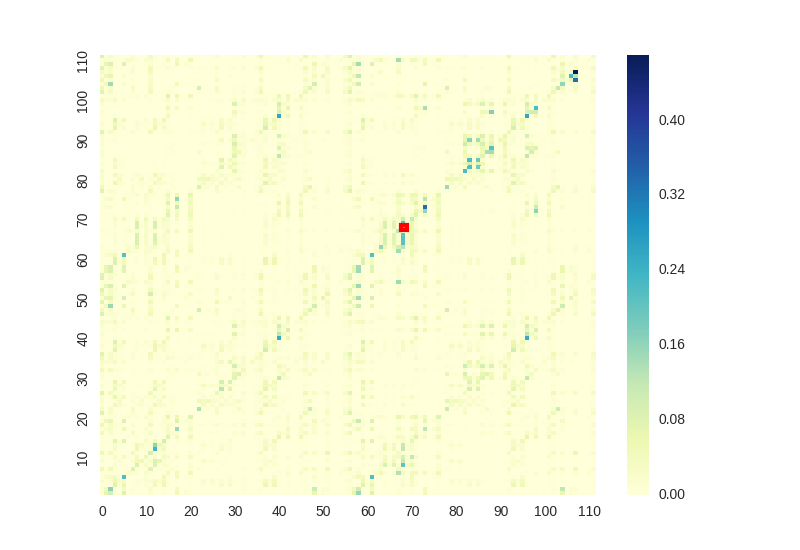
\includegraphics[scale=0.4]{../code-LOT-extension/plots/q-l30-a1-k5-l1-meFalse.png}
  \end{subfigure}
  ~
   \begin{subfigure}[b]{0.45\textwidth}
    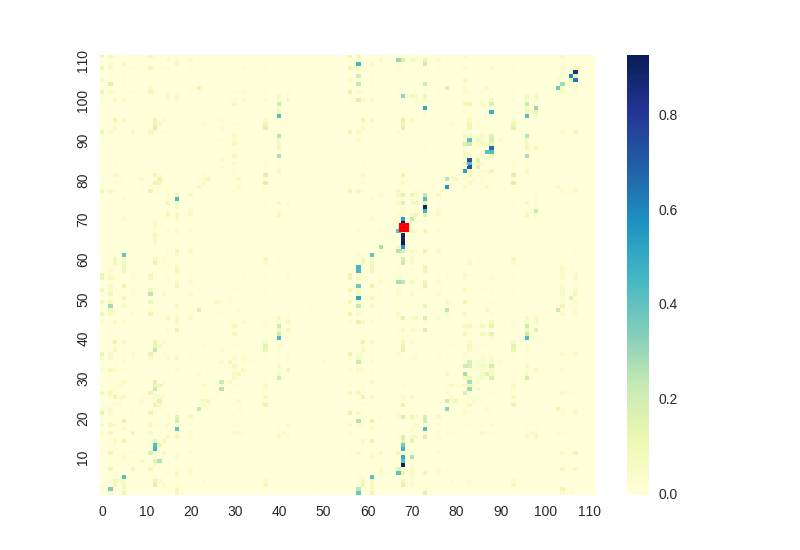
\includegraphics[scale=0.4]{../code-LOT-extension/plots/q-l30-a1-k5-l10-meFalse.png}
  \end{subfigure}
  \caption{$Q$-matrices for $\alpha = 1, \lambda = 30, k = 5$, $200$ samples per parent type with either $l = 1$ (left) and $l = 10$ (right). The boxed value corresponds to $P(t_{68} | t_{68})$. You have to zoom in all the way to see something. Otherwise; it's similar to the mutation value of our target in the reduced space}
  \label{fig:q-matrices}
\end{figure}

\newpage

Finally, we can see how the above affects actual applications of only replication, only mutation, and replication \emph{and} mutation using the matrices shown above. To construct these plots I took the mean top $3$ types from $1000$ simulations using either of the three dynamics. If $t_{68}$ was not in the top $3$, I took out the third most prolific type and added $t_{68}$ instead. 

\begin{figure}[h!]
  \centering
  \begin{subfigure}[b]{0.45\textwidth}
    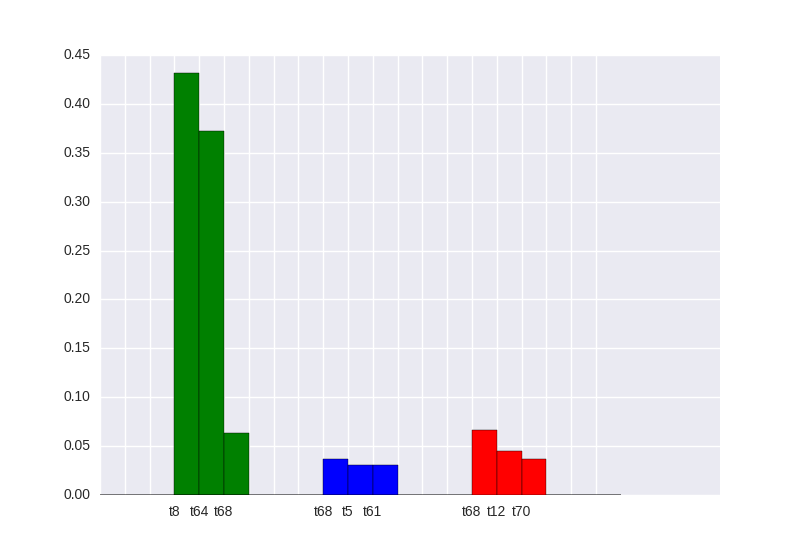
\includegraphics[scale=0.4]{../code-LOT-extension/plots/rmd-lam30-a1-k5-s200-l1-meFalse.png}
  \end{subfigure}
  ~
   \begin{subfigure}[b]{0.45\textwidth}
    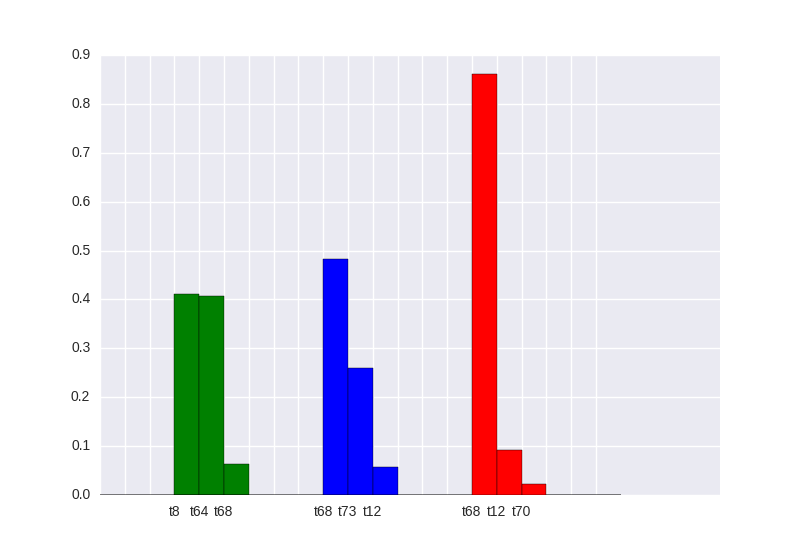
\includegraphics[scale=0.4]{../code-LOT-extension/plots/rmd-lam30-a1-k5-s200-l10-meFalse.png}
  \end{subfigure}
  \caption{Mean proportion of top $2/3$ types and target $t_{68}$ under replication only (green plot), mutation only (blue plot), and replication {\em and} mutation (red plot) after $50$ generations with $\alpha = 1, \lambda = 30, k = 5$, $200$ samples per parent type and $l = 1$ (left figure) and $l = 10$ (right figure).}
  \label{fig:outcomes}
\end{figure}







\bibliographystyle{plainnat}
\bibliography{./bounds-rmd}
\end{document}
